\documentclass[UTF8,a4paper,zihao=-4]{ctexart}

\usepackage[margin=2.4cm]{geometry}
\usepackage{graphicx}
\usepackage{booktabs}
\usepackage{amsmath}
\usepackage{array}
\usepackage{float}
\usepackage{caption}
\usepackage{enumitem}
\usepackage{tikz}
\usetikzlibrary{arrows.meta,positioning}
\usepackage[hidelinks]{hyperref}

\captionsetup{font=small,labelsep=quad}
\setlist{nosep,leftmargin=2em}
\renewcommand{\arraystretch}{1.25}
\hyphenation{Revit BIM HVACIDA}

\title{\heiti 面向地铁暖通设计的规范知识库与\\大模型工具调用方法及实现}
\author{韩学伟\\[2pt] \small 中铁第六勘察设计院集团有限公司电气化设计院分公司,天津}
\date{}

\begin{document}
\maketitle

\begin{abstract}
\noindent
大语言模型为设计软件提供了自然语言入口,但在工程场景中直接使用存在两类风险:一是模型可能编造规范条文与计算系数;二是模型一旦获得模型修改权限,误操作难以追溯。本文给出一套面向地铁暖通设计的知识库与工具调用方法,并在 Revit 插件中实现。方法把设计知识分为计算口径、规范条文与操作步骤三类,条目化存储并保留出处,检索不到时明确回复"不在范围内";模型不直接操作 Revit,而是通过进程内命令总线调用 7 条只读命令读取工程与模型数据,唯一的修改命令由"总开关 + 修改开关"两级控制,执行前弹 Revit 原生确认对话框,且不写带单位的数值参数。系统对未启用、无密钥、断网等情形一律不发起请求并给出可执行的替代路径。回归测试覆盖工具清单、开关拒绝、密钥隔离、断网降级与提示词约束等 20 余项,结果符合设计预期。本文的贡献是把"知识可溯源"与"操作可审计"作为大模型进入设计软件的前置条件,并给出可复用的实现方式。
\vspace{0.5em}

\noindent\textbf{关键词:} 大语言模型;检索增强生成;工具调用;规范知识库;BIM;暖通设计
\end{abstract}

\section{引言}

设计院的知识以三种形态存在:规范条文(国家标准与行业标准)、院内计算口径(公式文档与算例)、软件操作经验(在 Revit 里怎么选取空间、怎么导出图纸)。新员工要花很长时间才能把三者对应起来;即使是有经验的设计人,在赶图阶段也常为"这个系数取多少、这条条文在哪"中断工作。

大语言模型的出现让"用自然语言问工程问题"成为可能,但工程场景对错误零容忍:编造一条不存在的条文号,或把 1.2 的系数写成 1.5,都会进入施工图。已有工作分别从检索增强生成\cite{lewis2020rag}、推理与行动交替\cite{yao2022react}、工具学习\cite{schick2023toolformer}等方向提升模型的事实性与可操作性;BIM 领域也出现了基于大规模日志的命令推荐\cite{du2025bimcommand}与基于 API 的自动算量\cite{taghaddos2019}。这些工作证明了可行性,但落到设计院的生产软件,还需要回答三个工程问题:知识从哪来、答不出怎么办、模型能动手到什么程度。

本文给出一套面向地铁暖通设计的方法与实现。第 2 节回顾相关工作;第 3 节给出知识条目化、检索策略、工具调用与安全控制四项方法;第 4 节介绍系统实现;第 5 节报告功能与安全回归结果;第 6 节讨论局限并总结。

\section{相关工作}

检索增强生成(RAG)把参数化记忆与非参数化检索结合,在知识密集任务上改善了事实性并提供了出处\cite{lewis2020rag}。ReAct 让模型交替产生推理轨迹与动作,通过与环境交互减少幻觉\cite{yao2022react};Toolformer 让模型自学何时调用哪个 API\cite{schick2023toolformer}。这三条路线共同说明:模型本身不存储可靠的工程事实,事实应来自外部数据源,动作应通过受控接口完成。

在 BIM 场景,Du 等基于 320 亿行真实操作日志训练命令推荐模型,Recall@10 约 84\%\cite{du2025bimcommand},说明模型可以学习软件操作序列;Taghaddos 等用 API 自动完成按工作区的算量\cite{taghaddos2019}。但这些工作关注"预测下一步做什么",而非"回答一个具体的设计问题并给出出处",也较少讨论修改模型时的权限边界。

\section{方法}

\subsection{知识条目化}

知识库把设计知识拆成条目,每条包含分类、标题、正文、出处四个字段(图\ref{fig:kb})。分类有三种:

\begin{itemize}
\item \textbf{计算口径}:某类系统的公式链、系数取值与默认值,出处指向院内公式文档与算例;
\item \textbf{规范条文}:标准原文,出处给出标准号、条号与条文首页;
\item \textbf{操作步骤}:在插件与 Revit 中的操作路径,出处指向界面与按钮。
\end{itemize}

条目化带来两个直接好处:一是检索结果可以定位到"哪一条",而不是一段泛泛的回答;二是条目可以随文档修订单独更新,不必重训模型。当前内置 56 条,覆盖大系统负荷与排烟、六类小系统、水力计算、材料表、出图与数据存储。

\begin{figure}[H]
\centering
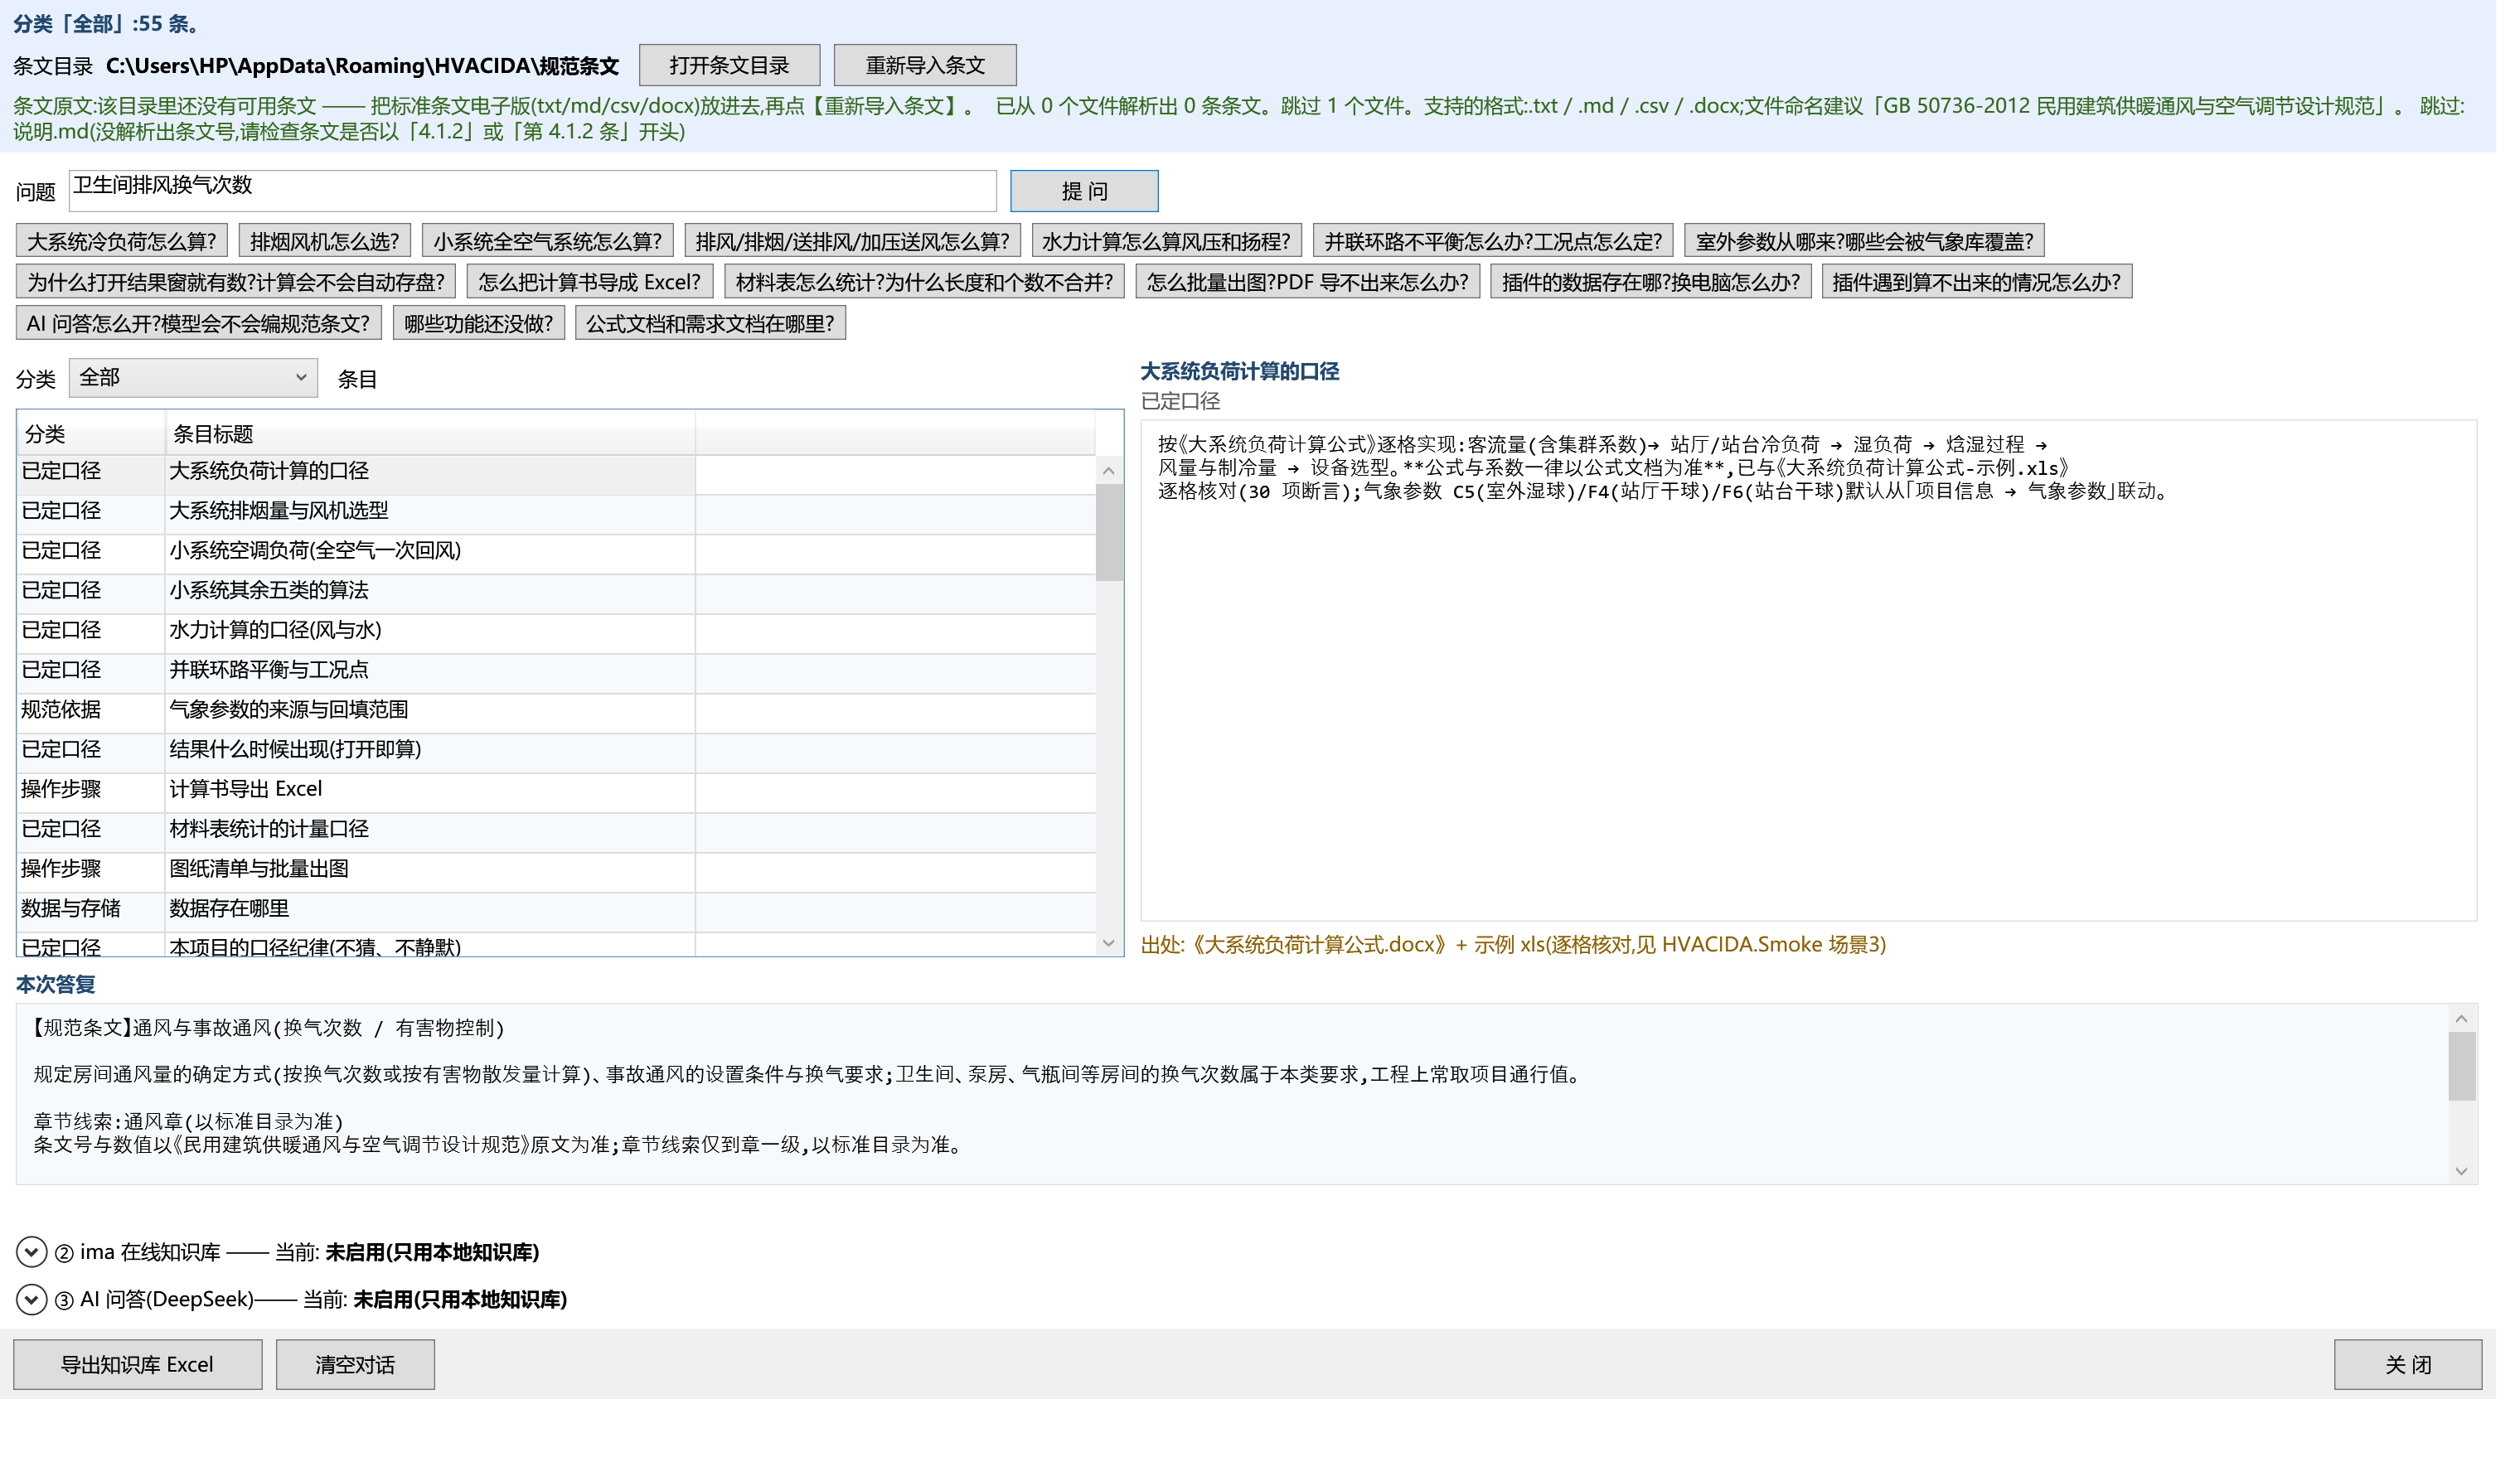
\includegraphics[width=0.95\textwidth]{figures/knowledge.png}
\caption{规范知识库窗:分类筛选、条目列表、正文与出处}\label{fig:kb}
\end{figure}

\subsection{检索与"答不出"}

检索采用"分类过滤 + 关键词命中 + 片段定位"三步:先按用户选择的分类缩小范围,再在标题与正文中做关键词匹配,命中处截取上下文作为答复的引用片段。对范围外的问题,系统不调用模型补全,而是明确回复"不在当前知识库范围内",并给出可执行的下一步(导入条文、换关键词或查看操作指南)。这一策略牺牲了一部分召回,换来的是"不编"。

标准条文支持从 txt、md、csv、docx 导入。导入时按"第 X 条""X.X.X"等格式切分条号,保留条号与原文;导入后的条目与内置条目同表检索,出处统一显示为标准号与条号。

\subsection{工具调用}

模型不直接访问 Revit API,而是通过进程内命令总线调用命令(图\ref{fig:flow})。总线维护一份命令表,每条命令带 JSON Schema 参数定义、是否修改模型的标记与说明文字;模型只能看到当前开关允许的命令,调用结果以 JSON 字符串回传,失败也返回结构化错误而不是抛异常。单轮对话最多 12 次工具调用,避免模型陷入循环。

\begin{figure}[H]
\centering
\resizebox{0.94\textwidth}{!}{%
\begin{tikzpicture}[
  node distance=0.55cm,
  box/.style={draw,rounded corners=2pt,minimum height=0.95cm,text width=2.9cm,align=center,font=\small},
  arr/.style={-{Stealth[length=2mm]},thick}
]
\node[box,fill=blue!6] (q) {设计问题};
\node[box,fill=green!6,right=of q] (kb) {知识库检索\\条目 + 出处};
\node[box,fill=orange!8,right=of kb] (llm) {大模型\\选择命令与参数};
\node[box,fill=gray!8,below=of llm] (bus) {命令总线\\开关 / 权限 / 审计};
\node[box,fill=gray!8,left=of bus] (cmd) {只读命令 7 条\\修改命令 1 条};
\node[box,fill=blue!6,left=of cmd] (ans) {答复 + 引用\\调用日志};

\draw[arr] (q) -- (kb);
\draw[arr] (kb) -- (llm);
\draw[arr] (llm) -- (bus);
\draw[arr] (bus) -- (cmd);
\draw[arr] (cmd) -- (ans);
\draw[arr,dashed] (ans.north) -- node[above,font=\scriptsize]{下一轮} (q.south);
\end{tikzpicture}}
\caption{知识检索与工具调用的处理流程}\label{fig:flow}
\end{figure}

命令集按"读取什么"划分(表\ref{tab:cmds}):工程信息、模型统计、空间列表、材料表、图纸清单、水力汇总、知识检索共 7 条只读命令;唯一的修改命令用于写参数,单独受第二级开关控制。

\begin{table}[H]
\centering
\caption{命令集与权限}\label{tab:cmds}
\small
\begin{tabular}{p{5.0cm}p{3.9cm}p{5.3cm}}
\toprule
命令 & 读取内容 & 权限 \\
\midrule
\texttt{get\_project\_info} & 工程名称、地点、阶段 & 只读 \\
\texttt{analyze\_model\_statistics} & 空间/墙/图纸数量 & 只读 \\
\texttt{list\_spaces} & 空间编号、名称、面积、层高 & 只读 \\
\texttt{get\_material\_takeoff} & 材料表归并结果 & 只读 \\
\texttt{list\_sheets} & 图纸清单与视图数 & 只读 \\
\texttt{get\_hydraulic\_summary} & 各系统阻力与需求值 & 只读 \\
\texttt{search\_knowledge} & 知识库条目与出处 & 只读 \\
\texttt{set\_parameter\_value} & 写构件参数 & 需两级开关 + 原生确认 \\
\bottomrule
\end{tabular}
\end{table}

\subsection{安全控制}

修改权限被拆成两级:第一级"启用 AI 对话"决定是否把工具清单下发给模型;第二级"允许模型修改模型"决定修改命令是否可见、可执行。两级都关闭时,模型看到的是空清单;只开第一级时,修改命令不下发,即使模型硬编码调用也会被总线拒绝。

执行修改前,插件弹出 Revit 原生确认对话框,默认按钮为"否",列出将要修改的构件数量;单次调用最多 200 个构件;带单位的数值参数一律不写,避免内部单位换算错误。每次调用都写入日志(命令名、参数摘要、耗时、成功或失败),对话窗口逐条显示,便于事后审计。

\subsection{密钥与降级}

接口密钥不落在明文配置中:密钥经 Windows DPAPI 加密后按工作区隔离存储,换一个工程取不到另一个工程的密钥;设置文件只记录"是否已配置"。未启用、未配置密钥、网络不可达三种情形下,系统都\textbf{不发起请求}:未启用时给出开关位置,未配置时提示去设置,断网时返回失败并说明"没有模型回答",同时保留本地知识库可用。

系统提示词对模型提出三条约束:回答前先取真实数据;禁止编造条文号与系数;修改模型前必须先征得确认。工具调用开启时,界面明确提示"工程数据会出网",把数据边界写在用户能看到的地方。

\section{系统实现}

AI 对话窗(图\ref{fig:ai})把对话、工具调用与设置放在同一窗口:顶部是两级开关与模型可见的工具数,中部是对话流,底部是输入框与发送按钮;每次工具调用在对话流下方逐条列出命令名、状态与耗时。知识库窗(图\ref{fig:kb})提供分类筛选、快捷问题、条目列表与正文,答复下方单列出处。

\begin{figure}[H]
\centering
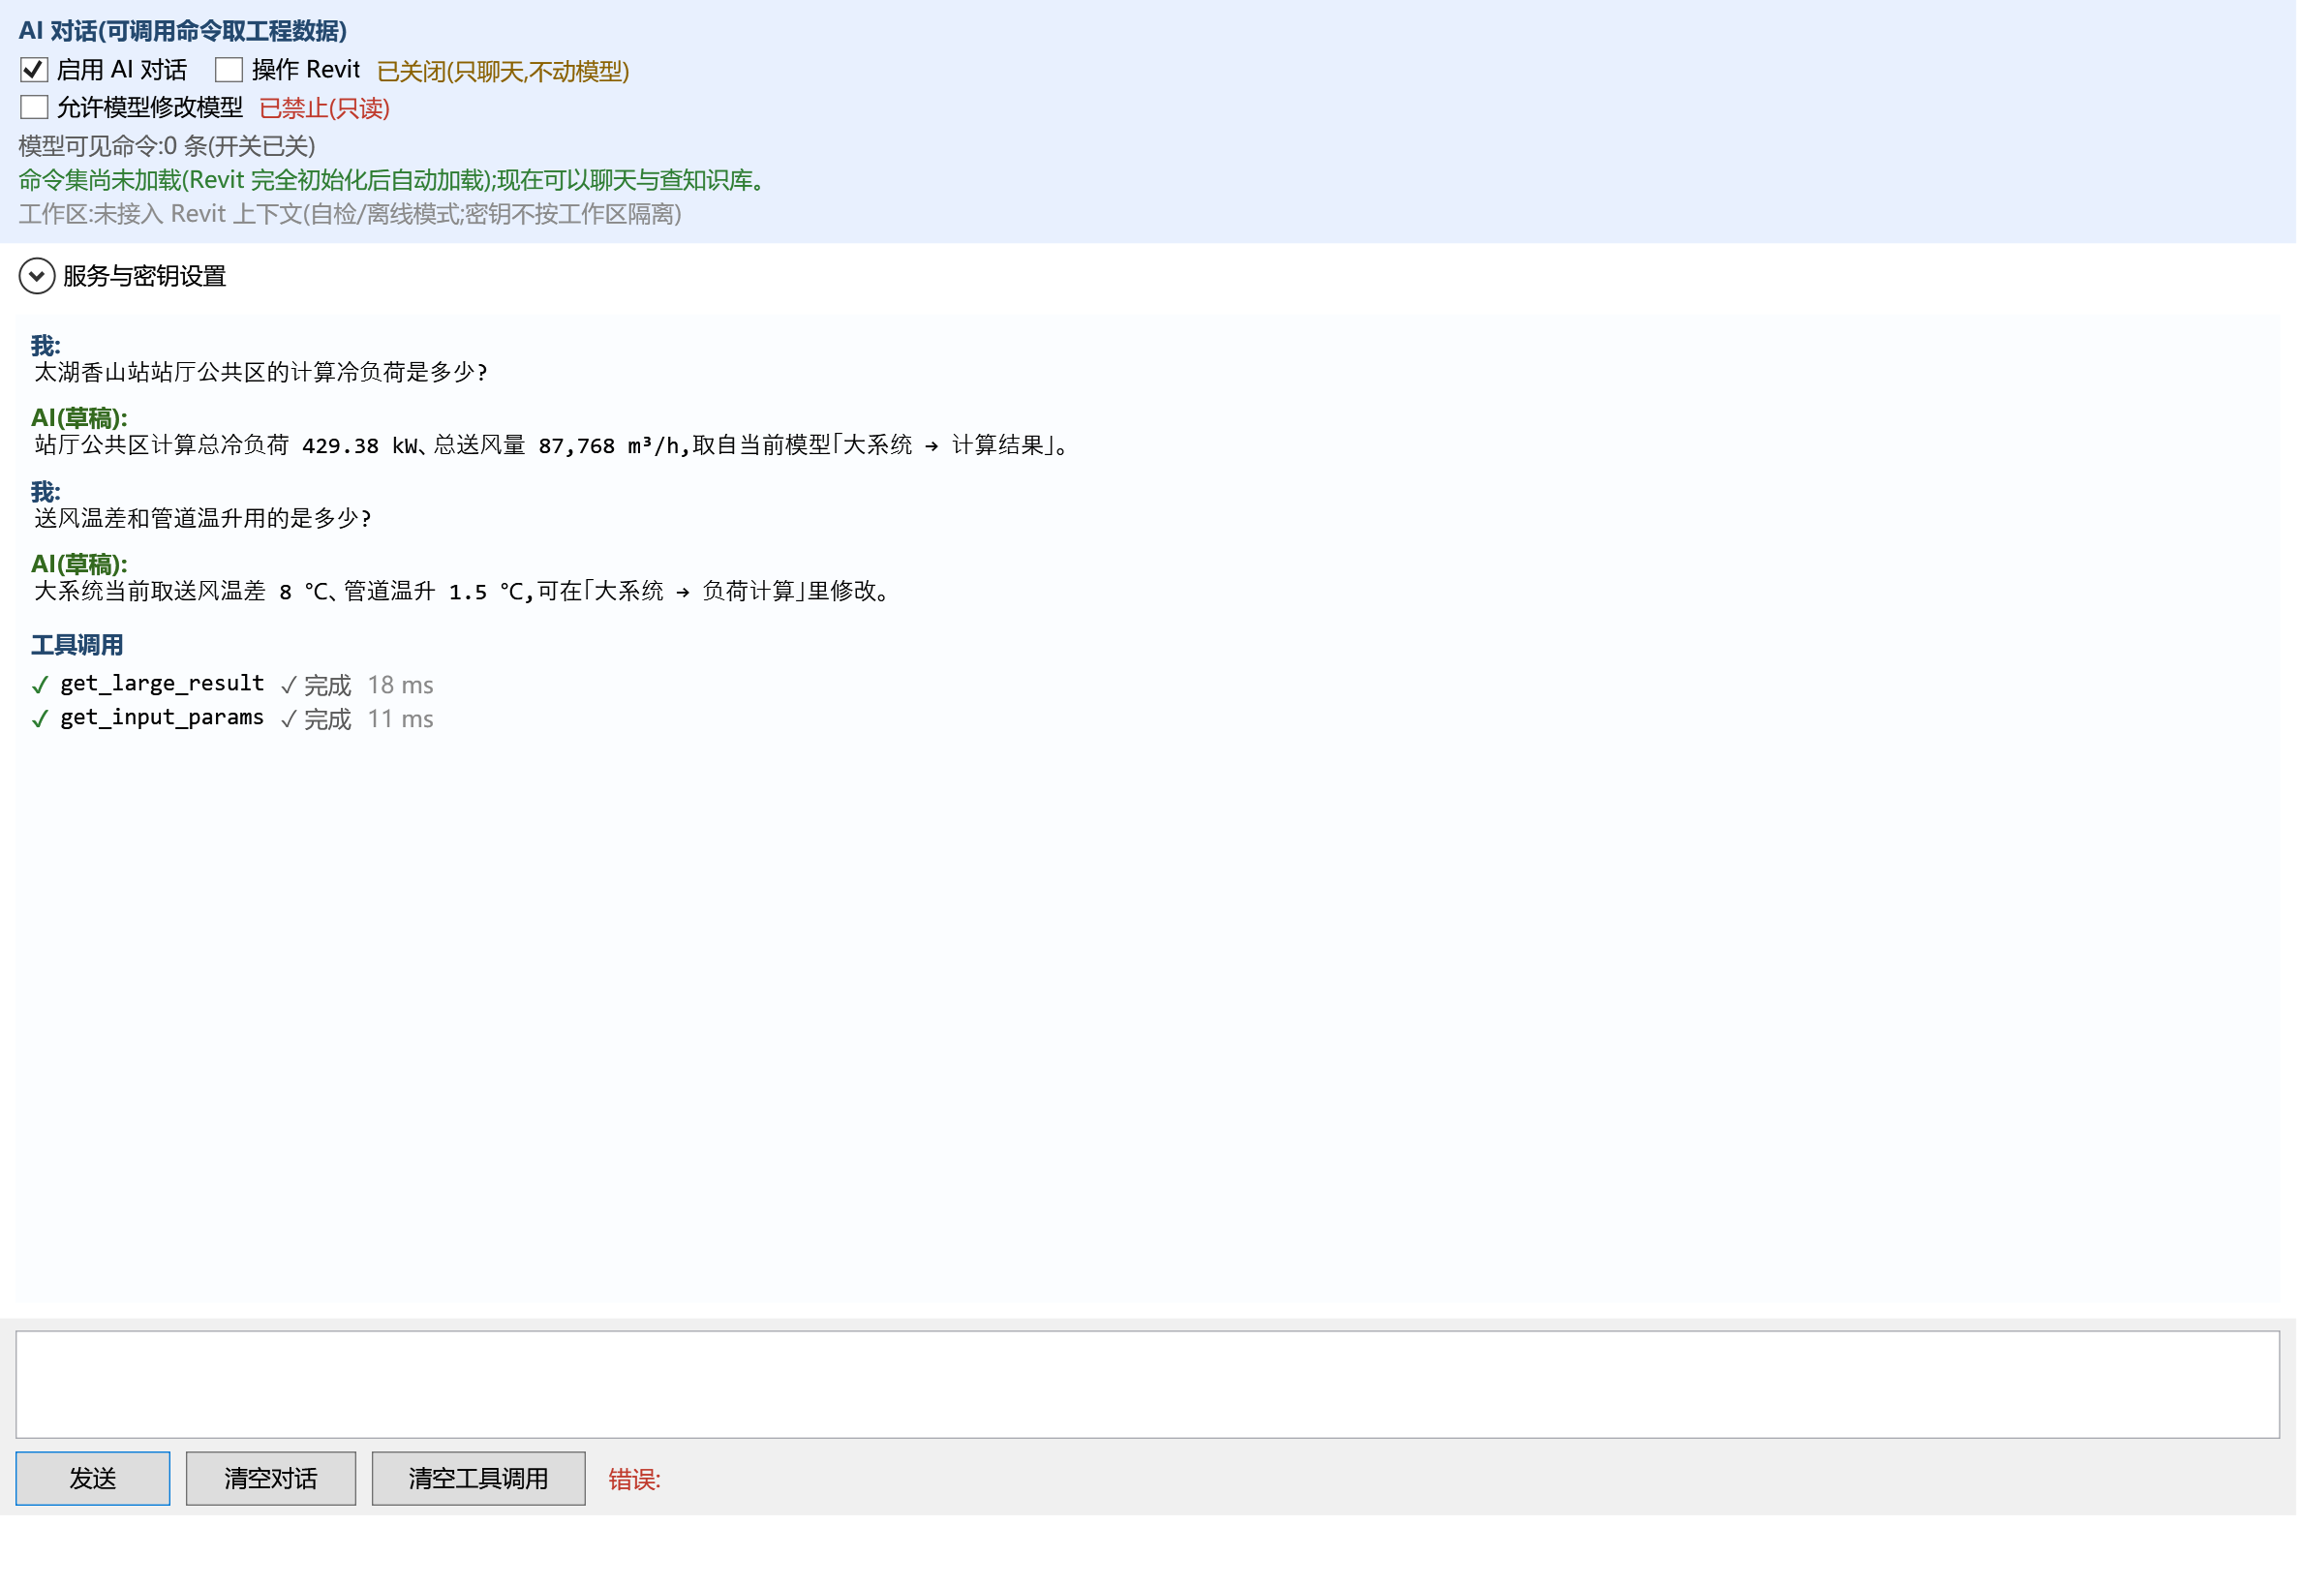
\includegraphics[width=0.9\textwidth]{figures/ai-chat.png}
\caption{AI 对话窗:两级开关、对话流与工具调用日志}\label{fig:ai}
\end{figure}

命令总线与知识库都在 Core 程序集中实现,不依赖 Revit;Revit 层只提供命令处理器(读取空间、写参数)并注册到总线。这样的分层使得总线、开关与密钥逻辑可以在无 Revit 的环境下用脚本回归,也让"拒绝执行"这类安全路径可以被测试覆盖。

\section{评估}

\subsection{功能与安全回归}

评估以可执行断言为主(表\ref{tab:tests}),覆盖四类行为:工具可见性、拒绝路径、密钥隔离、断网降级。所有用例在无 Revit 的环境下运行,结果与设计预期一致。

\begin{table}[H]
\centering
\caption{功能与安全回归用例(节选)}\label{tab:tests}
\small
\begin{tabular}{p{6.4cm}p{7.4cm}}
\toprule
用例 & 预期与结果 \\
\midrule
命令集未加载 & 总线不就绪,不下发任何工具 \\
总开关关闭 & 工具清单为空;硬调被拒绝 \\
仅开第一级 & 工具清单 7 条;修改命令不可见、不可执行 \\
两级都开 & 工具清单 8 条;修改命令可执行并留日志 \\
修改命令说明 & 写明会改模型、执行前确认、数值参数不写 \\
命令抛异常 & 返回结构化错误,不向界面抛出 \\
密钥存储 & 文件无明文;按工作区隔离;换工作区取不到 \\
未配置密钥 / 断网 & 不发起请求;回答为空并说明原因;不执行命令 \\
提示词约束 & 先取真实数据、禁编条文号与系数、改模型前确认 \\
\bottomrule
\end{tabular}
\end{table}

\subsection{知识覆盖}

内置 56 条覆盖了软件的全部功能面:每个面板至少一条口径条目与一条操作条目,规范条文按标准号与条号检索。以"卫生间排风换气次数"为例,检索返回规范条文条目(通风与事故通风)与院内口径条目(默认 6 次/h、卫生间常用 20 次/h),答复中同时给出两类出处,避免把"规范要求"与"院内取值"混为一谈。

\subsection{讨论}

本文的评估是功能与安全评估,不含模型回答质量的基准测试。原因有二:一是设计问题缺少公开标注集;二是同一问题在不同项目下的正确答案不同(取哪个系数取决于工程条件),用固定答案评测会误导。更合适的评估是"设计人是否愿意采纳",这需要在实际项目中做长期观察,暂不在本文范围内。

局限还包括:命令集只覆盖读取与写参数,尚不支持批量建模;知识库条目需要人工维护,文档修订后要同步更新;模型上下文只包含当前工程数据,跨项目经验尚未利用。

\section{结论}

本文把大模型进入设计软件的门槛归纳为两条:知识可溯源、操作可审计。方法上以条目化知识库提供出处,以受控命令总线隔离模型与模型数据,以两级开关和原生确认限制修改权限,以离线降级保证不可用时的可用性。在 Revit 插件中的实现与 20 余项回归表明,这些约束可以被工程化地落实,而不是停留在提示词层面。后续将扩展命令集(批量读取与建模)、引入回答质量的人工评价,并把知识条目与院内文档的版本管理打通。

\bibliographystyle{plain}
\bibliography{references}

\end{document}
